\vspace{1.25in}

\question
Use the following phylogenetic tree to answer the following questions.
\begin{center}
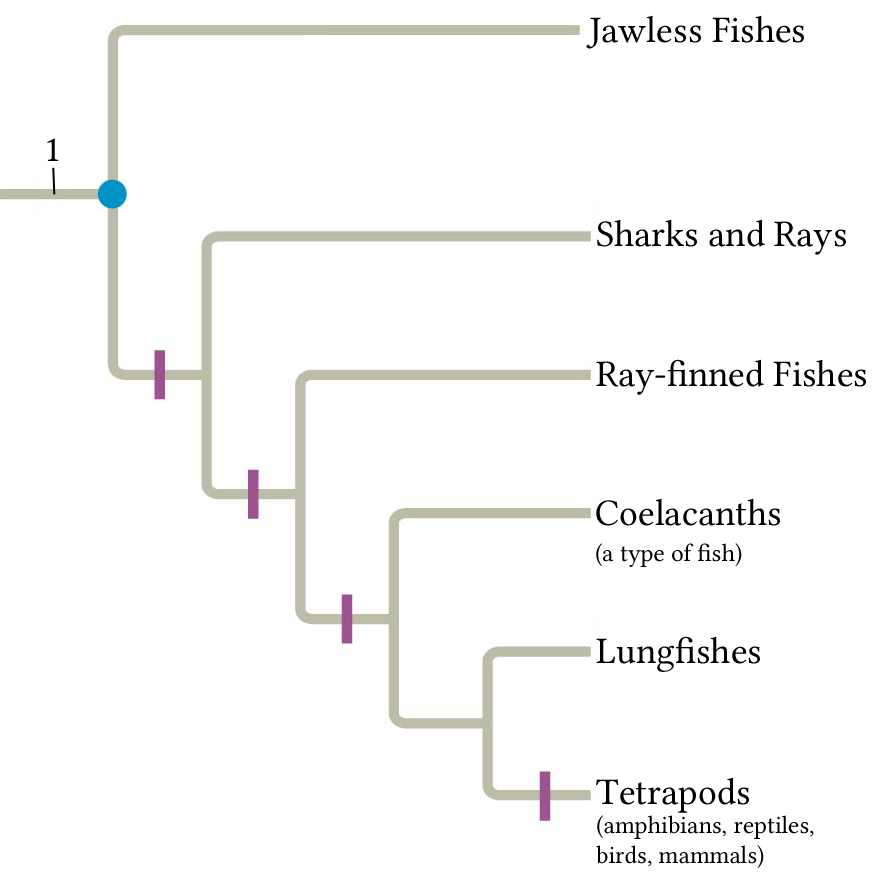
\includegraphics[width=0.4\textwidth]{vertebrate_phylogeny}
\end{center}

\begin{parts}
\part[5]
Are the coelacanths more closely related to ray-finned fishes or to tetrapods. Tell how you know.

\begin{minipage}[t][0.9in]{0.9\textwidth}%

\begin{solution}
Coelacanths are more closely related to tetrapods (2 pts) because they share a more recent common ancestor with tetrapods than ray-finned fishes (2 pts).
\end{solution}

\end{minipage}

\part[5]
Which group is a basal group (taxon)? What does this mean about it's evolution compared with that of the other groups? 

\begin{minipage}[t][0.9in]{0.9\textwidth}%
\begin{solution}
The jawless fishes are basal (2 pts). That means these fishes evolved before the other groups of fishes and tetrapods (2 pts).
\end{solution}
\end{minipage}

\part[5]
``Fishes'' includes all groups shown above except for tetrapods. Are fishes a monophyletic group? Tell how you know.

\begin{minipage}[t][0.9in]{0.9\textwidth}%
\begin{solution}
Fishes are not monophyletic (2 pts). Fishes contain some but not all of the descendants of the common ancestor (2 pts).
\end{solution}
\end{minipage}

\part[5]
What does the branch labeled ``1'' represent on this tree? What is the proper term for this branch?

%\begin{minipage}[t][0.6in]{\textwidth}%
\begin{solution}
The root (1 pt) represents the common ancestor of all groups shown on the phylogeny (2 pts). Grade only for 3 points.
\end{solution}
%\end{minipage}

\end{parts}
